\documentclass{article}
\usepackage[utf8x]{inputenc}
\usepackage[english,russian]{babel}
\usepackage{graphicx}
\usepackage{todonotes}
\usepackage{hyperref}
\begin{document}
\title{Расчёт прямой задачи для скалярного волнового уравнения по формуле Кирхгофа}
\author{\textbf{м.н.с. Голубев В.И.} \\ Лаборатория прикладной вычислительной геофизики МФТИ}
\maketitle
Рассмотрим задачу о распространении скалярного волнового поля в однородном нижнем полупространстве,
ограниченном сверху плоской поверхностью $S$.
Скалярное волновое уравнение во временной области может быть записано в виде:

\begin{equation}
\label{eq_wave_equation}
\nabla^2 P(\vec{r}, t) - \frac{1}{c^2}\frac{\partial^2}{\partial t^2}P(\vec{r}, t) = 0.
\end{equation}

Для него функция Грина имеет вид:
\begin{equation}
\label{eq_grin_function}
G^w(\vec{r}, t | \vec{r'}, t') = \frac{1}{4\pi|\vec{r} - \vec{r'}|}\delta(t - t' - \frac{|\vec{r} -
\vec{r'}|}{c}),
\end{equation}
где $\vec{r'}, t'$ - место расположения источника и время, в которое он начал действовать.

В общем виде (для ограниченной и для неограниченной области) формула Кирхгофа может быть записана
в виде:

\begin{equation}
\label{eq_kirchhoff_formula}
P(\vec{r'}, t') = \int_S \int_{-\infty}^{+\infty} [G^w(\vec{r'}, t' | \vec{r}, t) \frac{\partial}
{\partial n} P(\vec{r}, t) - P(\vec{r}, t) \frac{\partial}{\partial n} G^w(\vec{r'}, t' |
\vec{r}, t)] dt ds.
\end{equation}

Подставляя в (\ref{eq_kirchhoff_formula}) выражение для формулы Грина в явном виде (\ref{eq_grin_function}) получим
\begin{equation}
\label{eq_kirchhoff_homogeneous}
P(\vec{r'}, t') = \frac{1}{4\pi} \int_S [\frac{1}{c|\vec{r'} - \vec{r}|}
\frac{\partial |\vec{r'} - \vec{r}|}{\partial n}\frac{\partial P'}{\partial t'}
- \frac{\partial}{\partial n}(\frac{1}{|\vec{r'} - \vec{r}|}) P' + 
\frac{1}{|\vec{r'} - \vec{r}|}\frac{\partial}{\partial n}P'] ds,
\end{equation}
где $P' = P(\vec{r}, t' - \frac{|\vec{r'} - \vec{r}|}{c})$.

В нашем случае $\frac{\partial}{\partial n} = -\frac{\partial}{\partial z}$, поэтому выражение
(\ref{eq_kirchhoff_homogeneous}) может быть упрощено до вида:
\begin{equation}
\label{eq_kirchhoff_final}
P(\vec{r'}, t') = \frac{1}{4\pi} \int_S [\frac{z' - z}{|\vec{r'} - \vec{r}|}(\frac{1}{c}
\frac{\partial P'}{\partial t'} + \frac{1}{|\vec{r'} - \vec{r}|^2} P') - \frac{1}{|\vec{r'}
- \vec{r}|}\frac{\partial P'}{\partial z}] ds
\end{equation}

Пусть на поверхность полупространства воздействует давление в виде импульса Риккера:
\begin{equation}
\label{eq_ricker_wavelet}
P_{ricker} = P_0(1-2 \pi^2f^2t^2)e^{-\pi^2f^2t^2},
\end{equation}
тогда функция $P'(\vec{r'}, t')$ может быть записана в виде:
\begin{equation}
\label{eq_surface_pressure}
P'(\vec{r'}, t') = P(\vec{r}, t' - \frac{|\vec{r'} - \vec{r}|}{c}) = P_0(1-2 \pi^2f^2(t' - \frac{|\vec{r'} - \vec{r}|}{c})^2)e^{-\pi^2f^2(t'-\frac{|\vec{r'} - \vec{r}|}{c})^2}.
\end{equation}

С учётом (\ref{eq_ricker_wavelet}) аналитически могут быть получены значения
\begin{equation}
\label{eq_dp'_dt'}
\frac{\partial P'}{\partial t'} = -2\pi^2f^2P_0(3-2 \pi^2f^2(t' - \frac{|\vec{r'} - \vec{r}|}{c})^2)e^{-\pi^2f^2(t' - \frac{|\vec{r'} - \vec{r}|}{c})^2},
\end{equation}
и
\begin{equation}
\label{eq_dp'_dz}
\frac{\partial P'}{\partial z} = -2\pi^2f^2P_0(t' - \frac{|\vec{r'} - \vec{r}|}{c})[3-2 \pi^2f^2(t' - \frac{|\vec{r'} - \vec{r}|}{c})^2]e^{-\pi^2f^2(t' - \frac{|\vec{r'} - \vec{r}|}{c})^2}
\frac{z'-z}{c|\vec{r'}-\vec{r}|},
\end{equation}

Мною была реализована программа на языке Python, которая вычисляет численно интеграл (\ref{eq_kirchhoff_final}) методом прямоугольников с подстановкой (\ref{eq_dp'_dt'} и \ref{eq_dp'_dz}).
Проведён расчёт с $C_P = 2000$ м/с, $f = 10$ Гц.
На рисунках (\ref{img_snapshot_1} - \ref{img_snapshot_3}) представлено распределение $P$ по объёму (вертикальное сечение) в последовательные моменты времени.
При этом ось Z направлена вверх, т.е. граница области находится снизу.

\begin{figure}[ht]
  \center
  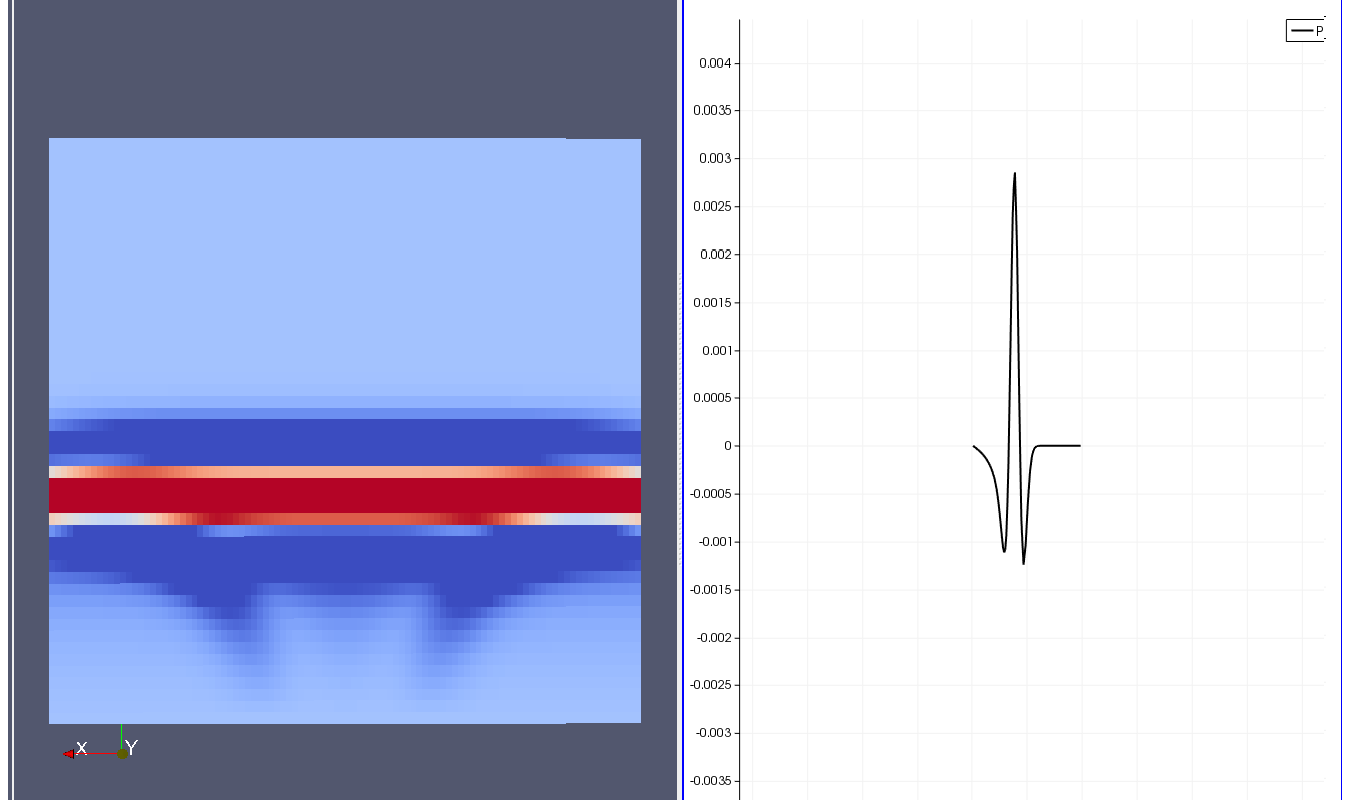
\includegraphics[scale=0.2]{pic_kirchhoff_scalar/t1.png}
  \caption{Через 100 мс}
\label{img_snapshot_1}
\end{figure}
\begin{figure}[ht]
  \center
  \caption{Через 100 мс}
  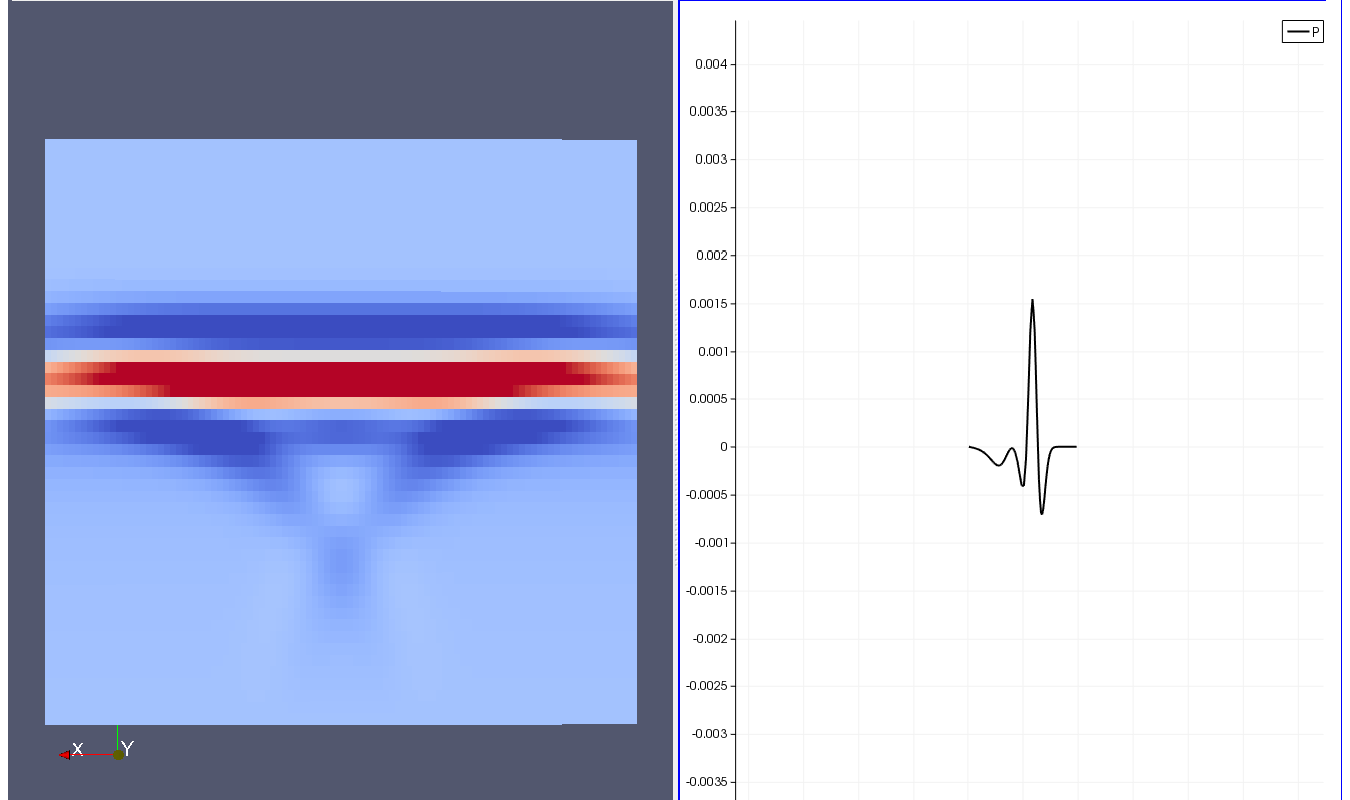
\includegraphics[scale=0.2]{pic_kirchhoff_scalar/t2.png}
  \caption{Через 200 мс}
\label{img_snapshot_2}
\end{figure}
\begin{figure}[ht]
  \center
  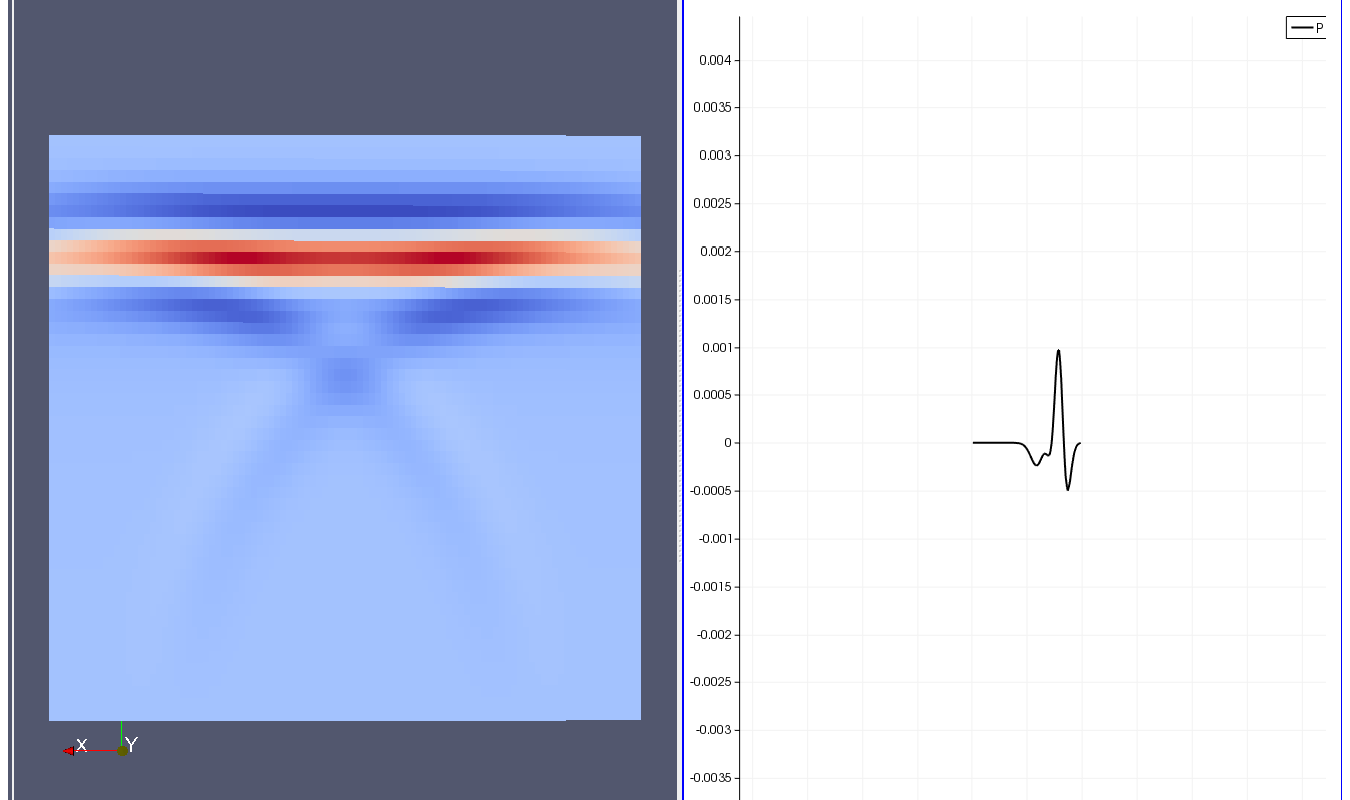
\includegraphics[scale=0.2]{pic_kirchhoff_scalar/t3.png}
  \caption{Через 300 мс}
\label{img_snapshot_3}
\end{figure}

Из особенностей результатов:
\begin{enumerate}
\item волна распространяется вдоль области и качественно сохраняет форму импульса;
\item от границы области распространяются артефакты - по-видимому, следствие того, что
в формуле Кирхгофа граница области - бесконечная прямая;
\item амплитуда сигнала затухает при распространении вглубь среды.
\end{enumerate}
\end{document}
